\documentclass[12pt]{IEEEtran}
\usepackage[scr]{rsfso}
\usepackage{amsmath}
\usepackage{pgfplots}
\usepackage{cmsrb}
\usepackage[OT2, T1]{fontenc}
\usepackage[serbian]{babel}
\usepackage{tikz}
\usepackage[justification=centering]{caption}
\usepackage{hyperref}
\usepackage{graphicx}
\usepackage{subcaption}
\usepackage{csquotes}

\pgfplotsset{compat=1.18}

\title{Digitalni upravlja\v{c}ki sistemi}
\author{Ra\v{c}unarski upravlja\v{c}ki sistemi}

\onecolumn
\numberwithin{equation}{subsection}
\numberwithin{figure}{section}

\begin{document}

\maketitle

\tableofcontents

\newpage
\section{\textbf{Kratko ponavljanje sistema automatskog upravljanja}}
\vspace{12pt}

\subsection{\textbf{Opis sistema i Laplasova transformacija}}
Sistemi kojima se bavimo na kursu su:

\begin{enumerate}
    \item \textbf{Linearni} - Sistemi za koje va\v{z}i princip \textbf{superpozicije} -
          ako je na pobudu $u_1$ odziv sistema $y_1$, a na pobudu $u_2$ odziv $y_2$, sistem
          je linearan ako va\v{z}i da, u slu\v{c}aju pobude $a_1u_1 + a_2u_2$, odziv izgleda kao
          $a_1y_1 + a_2y_2$ (u princip superpozicije su integrisani i principi \textbf{aditivnosti}
          i \textbf{homogenosti}).
    \item \textbf{Kauzalni} - Sistemi kod kojih odziv ne postoji prije
          dovo\dj{}enja pobudnog signala (dakle, prije po\v{c}etnog trenutka,
          njihova vrijednost je $0$).
    \item \textbf{Vremenski invarijantni} - Sistemi su vremenski invarijantni ako se parametri
          sistema ne mijenjaju u vremenu.
    \item \textbf{Stacionarni} - Dinami\v{c}ki sistemi sa koncentrisanim parametrima
          (opisuju se obi\v{c}nim diferencijalnim jedna\v{c}inama sa vremenom kao nezavisnom promjenljivom)
          koji su vremenski invarijantni nazivaju se stacionarnim sistemima.
\end{enumerate}

\vspace{12pt}

Pojednostavljenje analize sistema vr\v{s}imo konverzijom iz polja vremenskog
domena (diferencijalnih jedna\v{c}ina) u polje kompleksnih brojeva (algebarskih jedna\v{c}ina).
Stoga uvodimo \textbf{Laplasovu transformaciju}, koja se zapisuje kao

\begin{equation}
    Y(s) = \mathcal{L}\{y(t)\}
\end{equation}

Vezu izme\dj{}u ulaza i izlaza linearnih, vremenski kontinualnih, stacionarnih sistema opisuje se pomo\'{c}u
Laplasove transformacije \textbf{funkcijom prenosa}, odnosno

\begin{equation}
    G(s) = \frac{\mathcal{L}\{y(t)\}}{\mathcal{L}\{u(t)\}} = \frac{Y(s)}{U(s)}
\end{equation}

Dakle, \textbf{funckija prenosa je odnos Laplasovih transformacija izlaza i ulaza,
    pri nultim po\v{c}etnim uslovima}. Kod ovakvih sistema, one su \textbf{racionalne} (polinomi cijelih stepena se nalaze
i u brojiocu i u imeniocu) i va\v{z}i da je $n \geq m$, gdje je $n$ red polinoma (najve\'{c}i stepen) imenioca,
a $m$ red polinoma brojioca.

\subsection{\textbf{Modeliranje sistema}}
Sisteme kojima se bavimo na kursu (\textbf{linearne}) mo\v{z}emo modelovati:

\begin{enumerate}
    \item \textbf{Diferencijalnim jedna\v{c}inama}
    \item \textbf{Matemati\v{c}kim modelom u prostoru stanja}
\end{enumerate}

\vspace{12pt}

\textbf{Matemati\v{c}ki model u prostoru stanja} je opis sistema u formaciji

\begin{gather}
    \dot{x} = f(x, u)\\
    y = g(x, u)
\end{gather}

ili \v{c}es\'{c}e, matri\v{c}no

\begin{gather}
    \dot{x} = Ax + Bu\\
    y = Cx + Du
\end{gather}

gdje je $x$ \textbf{vektor promjenljivih stanja}, $u$ \textbf{ulazni signal},
dok je $y$ \textbf{izlaz iz sistema} (\textbf{odziv}).

Matrica $A$ se naziva \textbf{matrica stanja}, matrica $B$ \textbf{matricom ulaza}.
Matrica $C$ je \textbf{matrica izlaza}, dok je $D$ \textbf{matrica ulaza-izlaza}.

Ako uradimo Laplasovu transformaciju jedna\v{c}ine stanja i jedna\v{c}ine izlaza, dobijamo

\begin{gather}
    sX(s) = AX(s) + BU(s)\\
    Y(s) = CX(s) + DU(s)
\end{gather}

Uvr\v{s}tavanjem prve u drugu jedna\v{c}inu, dobijamo

\begin{gather}
    (sI - A)X(s) = BU(s)\\
    X(s) = (sI-A)^{-1}BU(s)\\
    Y(s) = (C(sI-A)^{-1}B + D)U(s)
\end{gather}

te se funkcija prenosa mo\v{z}e odrediti kao

\begin{equation}
    G(s) = C(sI - A)^{-1}B + D
\end{equation}

Inverzna matrica se odre\dj{}uje kao

\begin{equation}
    (sI - A)^{-1} = \frac{\text{adj}(sI - A)}{\det{(sI - A)}} = \frac{(\text{cof}(sI - A))^{T}}{\det{(sI - A)}}
\end{equation}

\subsection{\textbf{Linearizacija sistema}}
\textbf{Linearizacija sistema} su\v{s}tinski je potrebna pri analizi nelinearnih sistema,
nakon koje mo\v{z}emo primjeniti pretpostavke i zakone teorije upravljanja na linearne sisteme.
Linearizacija se vr\v{s}i \textbf{oko mirne radne ta\v{c}ke} (radno stanje
u kom proces mo\v{z}e ostati neograni\v{c}eno dugo ako na njega ne
djeluje poreme\'{c}aj).

Radne ta\v{c}ke procesa nalazimo kada su promjene sistema nulte, odnosno

\begin{equation}
    \dot{x} = f(x, u) = 0
\end{equation}

Odstupanja vrijednosti promjenljivih stanja i ulaza linearizovanog modela
od stvarnih vrijednosti pomenutih zapisa\'{c}emo kao

\begin{gather}
    x = x_{0} + \Delta{x}\\
    u = u_{0} + \Delta{u}
\end{gather}

Ako razvijemo prvu jedna\v{c}inu matemati\v{c}kog modela u prostoru stanja
($\dot{x} = f(x, u)$) u Tejlorov red u okolini mirne radne ta\v{c}ke koja
ima koordinate $(x_{0}, u_{0})$, zanemaruju\'{c}i izvode 
vi\v{s}eg reda od prvog, dobijamo slede\'{c}e:

\begin{equation}
    \dot{x} = \frac{d}{dt}{(x_{0} + \Delta{x})} = \frac{df(x, u)}{dt} = f(x_{0}, u_{0}) + \frac{\partial f(x_0, u_0)}{\partial x}(x - x_{0}) + \frac{\partial f(x_0, u_0)}{\partial u}(u - u_{0})
\end{equation}

U mirnoj radnoj ta\v{c}ki, va\v{z}i da je $f(x_{0}, u_{0}) = 0$, pa je

\begin{equation}
    \dot{\Delta{x}} = \frac{\partial f(x_{0}, u_{0})}{\partial x}\Delta{x} + \frac{\partial f(x_{0}, u_{0})}{\partial u}\Delta{u}
\end{equation}

Poslednja jedna\v{c}ina je \textbf{linearizovan matemati\v{c}ki model u prostoru stanja nelinearnog sistema}.

Sli\v{c}no, za $y = g(x, u)$, kao i za odziv $y_{0}$ kada je ulaz u sistem $u_0$
i vrijednosti promjenljivih stanja $x_{0}$ ($y_{0} = g(x_{0}, u_{0})$), dobijamo

\begin{gather}
    y = y_{0} + \Delta{y} = g(x, u) = g(x_{0}, u_{0}) + \frac{\partial g(x_{0}, u_{0})}{\partial x}\Delta{x} + \frac{\partial g(x_{0}, u_{0})}{\partial u}\Delta{u}\\
    \Delta{y} = \frac{\partial g(x_{0}, u_{0})}{\partial x}\Delta{x} + \frac{\partial g(x_{0}, u_{0})}{\partial u}\Delta{u}
\end{gather}

\begin{figure}[h]
    \centering
    \begin{tikzpicture}
        \begin{axis}[xmin=-1, xmax=5, ymin=-1, ymax=3,
                axis lines=middle, xticklabels=\empty, yticklabels=\empty,
                xlabel=$t$, ylabel=$y$]
            \addplot[red, thick, domain=0:5]{2*(1-e^-x)}
            node[left, yshift=-20px] {Nelinearan sistem};
            \addplot[blue, thick, domain=0:4.135]{0.545*x + 0.7465}
            node[left, xshift=-23px, yshift=-13px] {Linearna aproks.};
            \addplot[only marks, blue] coordinates {(1.3, 1.455)}
            node[above, xshift=-18px] {R. ta\v{c}ka};
        \end{axis}
    \end{tikzpicture}
    \caption{Crvenom bojom je ozna\v{c}en \textbf{nelinearan sistem},
        dok je plavom bojom ozna\v{c}ena \textbf{njegova linearna aproksimacija},
        kao i \textbf{radna ta\v{c}ka} oko koje linearizujemo.}
\end{figure}

\subsection{\textbf{Odzivi sistema prvog i drugog reda na razli\v{c}ite pobude}}

\textbf{Red sistema} odre\dj{}ujemo po tome koji je najve\'{c}i izvod funckije
koji se pojavljuje u diferencijalnoj jedna\v{c}ini koja ga opisuje (recimo, sistem
drugog reda sadr\v{z}i u sebi izvod najvi\v{s}e drugog reda, i sl.).

\begin{enumerate}
    \item
          Karakteristi\v{c}ni oblik \textbf{sistema prvog reda} je

          \begin{equation}
              \dot{y(t)} + ay(t) = bu(t)
          \end{equation}

          \textbf{Funkcija prenosa} ovakvog sistema je

          \begin{equation}
              G(s) = \frac{Y(s)}{U(s)} = \frac{b}{s + a}
          \end{equation}

          \begin{enumerate}
              \item
                    \textbf{Odziv sistema} na impulsni (Dirakov, \textit{delta impuls}) signal kao ulaz

                    \begin{equation}
                        u(t) = \delta(t) = \begin{cases}
                            0, \text{ , } t \neq 0 \\
                            +\infty \text{ , } t = 0
                        \end{cases}
                    \end{equation}

                    \v{c}ija je \textbf{Laplasova transformacija} $\mathcal{L}\{\delta(t)\} = 1$
                    jeste
                    \begin{gather}
                        Y(s) = G(s)U(s) = \frac{b}{s + a}\\
                        y(t) = \mathcal{L}^{-1}\{Y(s)\} = be^{-at}h(t)
                    \end{gather}

                    \begin{figure}[h]
                        \centering
                        \begin{tikzpicture}
                            \begin{axis}[xmin=-1, xmax=5, ymin=-1, ymax=3,
                                    axis lines=middle, xticklabels=\empty, yticklabels=\empty,
                                    xlabel=$t$, ylabel=$y$]
                                \addplot[blue, thick, domain=0:5, thick]{e^(-2*x)}
                                node[above, xshift=-30px] {$a > 0$};
                                \addplot[red, thick, domain=0:0.55, thick] {e^(2*x)}
                                node[below, xshift=20px] {$a < 0$};
                            \end{axis}
                        \end{tikzpicture}
                        \caption{\textbf{Plavom} je ozna\v{c}en slu\v{c}aj $a > 0$, dok je
                            \textbf{crvenom} ozna\v{c}en slu\v{c}aj $a < 0$.}
                    \end{figure}

                    \newpage
              \item
                    \textbf{Odziv sistema} na Hevisajdov signal kao ulaz

                    \begin{equation}
                        u(t) = h(t) = \begin{cases}
                            0 \text{ , } t < 0 \\
                            1 \text{ , } t \geq 0
                        \end{cases}
                    \end{equation}

                    \v{c}ija je Laplasova transformacija $\mathcal{L}\{h(t)\} = \frac{1}{s}$ je
                    \begin{gather}
                        Y(s) = G(s)U(s) = \frac{b}{s+a}\frac{1}{s} = \frac{\frac{b}{a}}{s} - \frac{\frac{b}{a}}{s + a}\\
                        y(t) = \mathcal{L}^{-1}\{Y(s)\} = \frac{b}{a}(1-e^{-at})h(t)
                    \end{gather}

                    \begin{figure}[h]
                        \centering
                        \begin{tikzpicture}
                            \begin{axis}[xmin=-1, xmax=5, ymin=-1, ymax=3,
                                    axis lines=middle, xticklabels=\empty, yticklabels=\empty,
                                    xlabel=$t$, ylabel=$y$]
                                \addplot[blue, thick, domain=0:5]{(1 - e^(-x))}
                                node[below, xshift=-20px] {$a > 0$};
                                \addplot[red, thick, domain=0:1.386]{e^x - 1}
                                node[above, xshift=20px, yshift=-20px] {$a < 0$};
                                \addplot[dashed] {1} node [pos=0.45, above left] {$\frac{b}{a}$};
                            \end{axis}
                        \end{tikzpicture}
                        \caption{\textbf{Plavom} je ozna\v{c}en slu\v{c}aj $a > 0$, dok je
                            \textbf{crvenom} ozna\v{c}en slu\v{c}aj $a < 0$.}
                    \end{figure}

          \end{enumerate}
          \newpage
    \item
          Karakteristi\v{c}ni oblik \textbf{sistema drugog reda} je

          \begin{equation}
              \ddot{y(t)} + a\dot{y(t)} + by(t) = cu(t)
          \end{equation}

          \textbf{Funkcija prenosa} ovakvog sistema je

          \begin{equation}
              G(s) = \frac{Y(s)}{U(s)} = \frac{c}{s^2 + as + b}
          \end{equation}

          ili \v{c}e\v{s}\'{c}e zapisano

          \begin{equation}
              G(s) = \frac{K\omega_{n}^2}{s^2 + 2\xi\omega_{n}s + \omega_{n}^2}
          \end{equation}

          \textbf{Polovi sistema} su

          \begin{equation}
              p_{1, 2} = -\xi\omega_{n} \pm j\omega_{n}\sqrt{1 - \xi^2} = -\sigma \pm j\omega
          \end{equation}

          \textbf{Step odziv} sistema drugog reda izgleda

          \begin{equation}
              y(t) = \left(1 - e^{-\xi\omega_{n}t}\frac{1}{\sqrt{1 - \xi^2}}\sin{(\omega_{n}\sqrt{1-\xi^2}t + \phi)}\right)h(t)
          \end{equation}

          \begin{figure}[h]
              \centering
              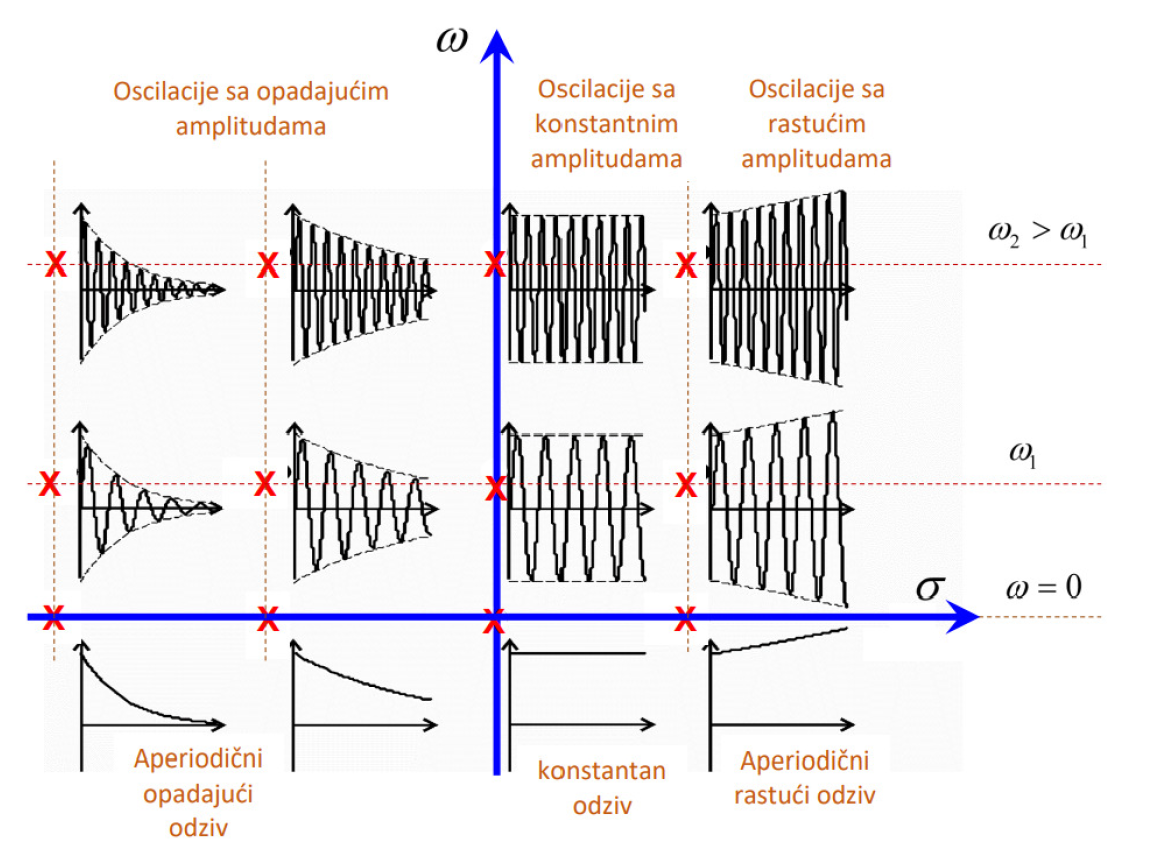
\includegraphics[width=0.7\textwidth]{Pictures/Screenshot 2023-10-21 213251.png}
              \caption{Razli\v{c}iti odzivi u zavisnosti od parametara $\omega_{n}$ i $\xi$, na $\delta$ pobudu.}
          \end{figure}

\end{enumerate}

\newpage

\subsection{\textbf{Karakteristike sistema automatskog upravljanja}}

\begin{enumerate}
    \item \textbf{Stati\v{c}ko poja\v{c}anje} - Dobija se izrazom

          \begin{equation}
              K_{stat} = \lim_{t \to 0}G(s) = G(0)
          \end{equation}

    \item \textbf{Dominantna vremenska konstanta} - Govori o tome koliko brzo
          \'{c}e sistem u\'{c}i u ustaljeno stanje. Dobija se izrazom

          \begin{equation}
              T_{d} = \frac{1}{|\sigma_{d}|}
          \end{equation}

          gdje je $\sigma_{d}$ realni dio dominantnog pola (pola najbli\v{z}eg imaginarnoj osi).

    \item \textbf{Gre\v{s}ka u ustaljenom stanju} -Govori o tome koliko
          ostvarena vrijednost odziva sistema prati \v{z}eljenu (referentnu) vrijednost procesa.

    \item \textbf{Stabilnost sistema} - Govori o tome \v{s}ta se de\v{s}ava sa sistemom
          kada se on izvede iz mirne radne ta\v{c}ke (u smislu Ljapunova). Stabilnost zavisi od 
          polo\v{z}aja polova funkcije prenosa.

    \item \textbf{Brzina sistema} - Povezana sa \textbf{dominantnom vremenskom konstantom} i 
    odre\dj{}ena je polom najbli\v{z}im $Im$ osi. To je ujedno i \textbf{najsporiji pol} (\textbf{najsporija komponenta} odziva),
    pa iz toga proizilazi da je \textbf{sistem onoliko brz koliko je brza njegova najsporija komponenta}.
    Pri projektovanju regulatora, mogu\'{c}e je pomjeriti polove lijevo te tako ubrzati sistem, 
    ali kao posljedicu toga dobijamo preskoke i pro\v{s}irujemo propusni opseg funckije prenosa.

\end{enumerate}

\subsection{\textbf{Gre\v{s}ka u ustaljenom stanju}}

Gre\v{s}ka u ustaljenom stanju je pojava odstupanja ostvarene vrijednosti ($y(t)$) od \v{z}eljene vrijednosti ($r(t)$)
odziva sistema. Ona govori o sposobnosti sistema da prati \v{z}eljenu vrijednost
i defini\v{s}e se kao

\begin{gather}
    e_{ss} \stackrel{\text{def}}{=} \lim_{t \to \infty}{e(t)} = \lim_{s \to 0}{sE(s)}\\
    e(t) = r(t) - y(t)
\end{gather}

\textbf{Funkcija prenosa} od reference $R(s)$ do gre\v{s}ke $E(s)$ je

\begin{equation}
    E(s) = \frac{1}{1 + G(s)}R(s)
\end{equation}

Dakle, vidimo da gre\v{s}ka zavisi ne samo od prirode sistema, ve\'{c} i od
reference (pobude).

\textbf{Funkcija prenosa} bilo kojeg sistema mo\v{z}e se zapisati kao

\begin{gather}
    G(s) = \frac{K\prod\limits_{i=1}^{m}{(s - z_{i})}}{s^{N}\prod\limits_{j=1}^{n}{(s - p_{j})}} \text{ , } p_{j} \neq 0\\
    N + n \geq m
\end{gather}

gdje je $N$ red astatizma.

Defini\v{s}imo \textbf{stati\v{c}ko poja\v{c}anje glavne grane} kao

\begin{equation}
    K_{dc} = \lim_{s \to 0}{\left(\frac{K\prod\limits_{i=1}^{m}{(s - z_{i})}}{\prod\limits_{j=1}^{n}{(s - p_{j})}}\right)} \text{ , } p_{j} \neq 0
\end{equation}

Posmatrajmo gre\v{s}ku u ustaljenom stanju u odnosu na pobudni signal:

\begin{enumerate}
    \item \textbf{Pobuda je $r(t) = h(t)$}

          Tada je $R(s) = \frac{1}{s}$, te je gre\v{s}ka u ustaljenom stanju

          \begin{equation}
              e_{ss} = \lim_{s \to 0}{sE(s)} = \lim_{s \to 0} \frac{s \cdot \frac{1}{s}}{1 + G(s)} = \lim_{s \to 0}{\frac{1}{1 + G(s)}}
          \end{equation}

          Po definiciji, gre\v{s}ka u ustaljenom stanju na \textbf{step pobudu} jeste

          \begin{equation}
              e_{ss} \stackrel{\text{def}}{=} \frac{1}{1 + K_{p}}
          \end{equation}

          gdje se $K_{p}$ naziva \textbf{poziciona konstanta}.

          Ako je red astatizma $N = 0$, tada su vrijednosti gre\v{s}ke 
          u ustaljenom stanju i pozicione konstante

          \begin{gather}
              e_{ss} = \lim_{s \to 0}{\frac{1}{1 + G(s)}} = \frac{1}{1 + K_{dc}}\\
              K_{p} = \lim_{s \to 0}{G(s)} = K_{dc}
          \end{gather}

          Dakle, ako \textbf{nema astatizama} u sistemu, na \textbf{step ulaz
          uvijek \'{c}emo imati gre\v{s}ku u ustaljenom stanju}
          (ona nikada ne\'{c}e biti nula). Gre\v{s}ku mo\v{z}emo
          smanjiti jakim poja\v{c}anjem, no sistem tada trpi ve\'{c}e
          optere\'{c}enje.

          \vspace{12pt}

          Ako je red astatizma $N \geq 1$, tada je gre\v{s}ka u ustaljenom stanju

          \begin{gather}
              e_{ss} = \lim_{s \to 0}{\frac{1}{1 + G(s)}} = \lim_{s \to 0}{\frac{1}{1 + \frac{G_{0}(s)}{s^{N}}}} = \lim_{s \to 0}{\frac{s^{N}}{s^{N} + G_{0}(s)}} = 0\\
              K_{p} = \lim_{s \to 0}{G(s)} = \lim_{s \to 0}{\frac{G_{0}(s)}{s^{N}}} = \infty
          \end{gather}

          gdje je $G_{0}(s)$ funkcija prenosa sistema bez astatizama.

          Dakle, potreban je \textbf{bar jedan astatizam} u sistemu \textbf{kada je ulaz Hevisajdova funkcija} kako bi se poni\v{s}tila
          gre\v{s}ka u ustaljenom stanju.

          \vspace{12pt}

    \item \textbf{Pobuda je $r(t) = th(t)$}

          Tada je $R(s) = \frac{1}{s^{2}}$, te je gre\v{s}ka u ustaljenom stanju

          \begin{equation}
              e_{ss} = \lim_{s \to 0}{\frac{s \cdot \frac{1}{s^{2}}}{1 + G(s)}} = \lim_{s \to 0}{\frac{1}{s + sG(s)}} = \lim_{s \to 0}{\frac{1}{sG(s)}}
          \end{equation}

          Po definiciji, gre\v{s}ka u ustaljenom stanju na \textbf{rampa pobudu} jeste

          \begin{equation}
              e_{ss} \stackrel{\text{def}}{=} \frac{1}{K_{v}}
          \end{equation}

          gdje se $K_{v}$ naziva \textbf{brzinska konstanta}.

          \vspace{12pt}

          Analizom prethodne jedna\v{c}ine posti\v{z}u se slede\'{c}i rezultati:

          \begin{enumerate}
              \item Za $N = 0$, $K_{v} = 0$ i $e_{ss} \to \infty$
              \item Za $N = 1$, $K_{v} = K_{dc}$ i $e_{ss} = \frac{1}{K_{dc}}$
              \item Za $N \geq 2$, $K_{v} \to \infty$ i $e_{ss} \to 0$
          \end{enumerate}

          \vspace{12pt}

          Dakle, za otklanjanje gre\v{s}ke u ustaljenom stanju na \textbf{rampa pobudu},
          potrebno je \textbf{bar dva astatizma} u sistemu.

\end{enumerate}

\vspace{12pt}

Kada je u pitanju projektovanje regulatora, broj astatizama (integratora)
koje mo\v{z}e sadr\v{z}ati regulator ne prelazi $2$, jer se dodavanjem
ve\'{c} dva astatizma sistem dovodi na granicu stabilnosti.

\subsection{\textbf{Stabilnost sistema}}

Kroz teoriju upravljanja (linearnih) sistema pro\v{z}ima se pitanje - da li je
sistem stabilan? Ako sistem nije stabilan, nema smisla analizirati dodatne
karakteristike sistema kao \v{s}to su pona\v{s}anje u prelaznom re\v{z}imu,
gre\v{s}ka u ustaljenom stanju i dr.

\textbf{Stabilnost u smislu Ljapunova} defini\v{s}e se na na\v{c}in da je
mirna radna ta\v{c}ka stabilna ukoliko za svako pozitivno $\epsilon$ postoji
pozitivan broj $\delta(\epsilon)$ takav da ukoliko je po\v{c}etno stanje procesa
udaljeno od ravnote\v{z}nog stanja manje od $\delta$, tada \'{c}e cjelokupna
naredna trajektorija procesa biti unutar $\epsilon$-okoline ravnote\v{z}nog stanja,
odnosno

\begin{equation}
    ||x(0) - x_{0}|| < \delta \implies ||x(t) - x_{0}|| < \epsilon \text{ , } \forall t > 0
\end{equation}

\textbf{Asimptotska stabilnost} govori o tome da je radna ta\v{c}ka asimptotski
stabilna ukoliko je stabilna u smislju Ljapunova, te ukoliko se nakon dovoljno malog
poreme\'{c}aja asimptotski vra\'{c}a u ravnote\v{z}no stanje. Matemati\v{c}ki
zapisano,

\begin{equation}
    ||x(0) - x_{0}|| < \delta \implies \lim_{t \to \infty}{x(t)} = x_{0}
\end{equation}

Pored Ljapunovih uslova stabilnosti (koji su uop\v{s}tenje za bilo koju vrstu
sistema, bili oni linearni ili nelinearni), tako\dj{}e mo\v{z}emo razmatrati
\textbf{polove sistema}. Naime, \textbf{ako se svi polovi funkcije spregnutog prenosa sistema}
(\textbf{funkcija prenosa sistema} kada se zatvori negativna povratna sprega, dok se polovi
nalaze rje\v{s}avanjem jedna\v{c}ine $1 + G(s)H(s) = 0$) \textbf{nalaze lijevo od
imaginarne ose}, tada je linearni sistem \textbf{stabilan}. Bar jedan pol sa desne
strane imaginarne ose tjera sistem u \textbf{nestabilnost}, dok su \textbf{grani\v{c}no
stabilni} oni sistemi sa polovima na imaginarnoj osi kompleksne ravni. Va\v{z}no je 
napomenuti da su sistemi nestabilni i u slu\v{c}aju kada postoje \textbf{vi\v{s}estruki polovi}
na imaginarnoj osi (dva ili vi\v{s}e pola u jednoj istoj ta\v{c}ki).

U slu\v{c}aju da polovi sistema nisu poznati, mo\v{z}emo iskoristiti \textbf{Nikvisov kriterijum}.
\textbf{Funkcija spregnutog prenosa} sistema je

\begin{gather}
    W_{sp}(s) = \frac{G(s)}{1 + G(s)H(s)} = \frac{G(s)}{1 + W_{p}(s)}\\
    W_{p}(s) = G(s)H(s)
\end{gather}

gdje je $W_{p}(s)$ \textbf{funkcija povratnog prenosa}.

Obuhvatimo konturom $\mathcal{C}$ sve \textbf{polove} ($P$) i \textbf{nule} ($N$)
funckije $F(s) = 1 + W_{p}(s) = 1 + G(s)H(s)$
koji se nalaze u desnoj poluravni kompleksne ravni (ta kontura je beskona\v{c}an polukrug).
Znaju\'{c}i da stabilnost sistema \textbf{zavisi od nula} $F(s)$ (da ona \textbf{ne smije imati nule} u desnoj poluravni)
i pod pretpostavkom Ko\v{s}ijeve teoreme koja
govori da broj obuhvata preslikane krive oko koordinatnog po\v{c}etka iznosi
$N - P$, dolazimo do zaklju\v{c}ka da \textbf{obuhvat krive dobijene funkcijom $F(s)$
    oko koordinatnog po\v{c}etka mora biti jednak $-P$, da bi sistem bio stabilan}.
Prakti\v{c}no se uzima u obzir funkcija $W(s)$, te se gleda obuhvat oko ta\v{c}ke
$(-1, 0j)$.

\newpage
\section{\textbf{Dvopolo\v{z}ajni regulator i osnovni oblik kontinualnog PID regulatora}}

Sistem koji od sada posmatramo izgleda kao

\begin{figure}[h]
    \centering
    \begin{tikzpicture}
        \draw[->] (0, 0) node[left] {$r(t)$} -- (1, 0) {};
        \draw (1.25, 0) circle (0.25);
        \draw[->] (1.5, 0) node[above, xshift=12px] {$e(t)$} -- (2.5, 0) {};
        \draw (2.5, -0.5) rectangle (4.5, 0.5) node[pos=0.5] {Reg.};
        \draw[->] (4.5, 0) -- (5, 0) {};
        \draw (5.25, 0) circle (0.25);
        \draw[->] (5.25, 1) node[right] {$l(t)$ - poreme\'{c}aj} -- (5.25, 0.25) {};
        \draw[->] (5.5, 0) -- (6, 0) {};
        \draw (6, -0.5) rectangle (8, 0.5) node[pos=0.5] {Sistem};
        \draw (8, 0) node[right, xshift=58px] {$y(t)$} -- (10, 0) {};
        \draw[->] (9, 0) -- (9, -1.5) -- (5.5, -1.5) {};
        \draw (5.25, -1.5) circle (0.25);
        \draw[->] (5.25, -2.5)  node[right] {$n(t)$ - \v{s}um mjerenja} -- (5.25, -1.75) {};
        \draw[->] (5, -1.5) -- (1.25, -1.5) -- (1.25, -0.25) {};
    \end{tikzpicture}
    \caption{Kontinualni sistem koji posmatramo.}
\end{figure}

\subsection{\textbf{Dvopolo\v{z}ajni regulator}}

\textbf{Dvopolo\v{z}ajni regulatori} predstavljaju najjednostavnije
konvencionalne regulatore kod kojih se na osnovu znaka signala gre\v{s}ke
opredjeljuje za jedno od dva mogu\'{c}a izlazna stanja - $u_{min}$ i $u_{max}$.
Formalno zapisano,

\begin{equation}
    u(t) = \begin{cases}
        u_{min} \text{ , } e(t) < 0 \\
        u_{max} \text{ , } e(t) > 0
    \end{cases}
\end{equation}

Naj\v{c}e\v{s}\'{c}e, ova dva stanja se nazivaju \textbf{OFF} i \textbf{ON}
stanje, a sam regulator \textbf{ON}-\textbf{OFF regulatori}
(ili nekada \textbf{\textit{bang}} - \textbf{\textit{bang}}).

\begin{figure}[h]
    \centering
    \begin{tikzpicture}
        \begin{axis}[xmin=-2, xmax=2, ymin=-3, ymax=3,
                axis lines=middle, xticklabels=\empty, yticklabels=\empty,
                xlabel=$t$, ylabel=$u$]
            \addplot[blue, thick, domain=-2:0]{-2}
            node[right] {$u_{min}$};
            \addplot[blue, thick, domain=0:2]{2}
            node[left, xshift=-98px] {$u_{max}$};
            \draw[blue, thick] (axis cs:0, -2) -- (axis cs:0, 2) {};
        \end{axis}
    \end{tikzpicture}
    \caption{Osnovna implementacija dvopolo\v{z}ajnog regulatora.}
\end{figure}

Ovakvi regulatori i njihova prakti\v{c}no jednostavna upravlja\v{c}ka
strategija nalaze aplikacije u ku\'{c}noj automatici (regulacija temperature
sobe, rerne i sl.).

Me\dj{}utim, problem kod dvopolo\v{z}ajnih regulatora u njihovoj osnovnoj
implementaciji ogleda se u tome \v{s}to, nakon \v{s}to odziv dostigne \v{z}eljenu
vrijednost (recimo, regulacija temperature u sobi), pri ponovnom pojavljivanju
gre\v{s}ke u pra\'{c}enju referentne vrijednosti (ponovni pad temperature),
dolazi do instantne reakcije regulatora (koji vra\'{c}a
temperaturu na \v{z}eljenu vrijednost), te kako se ovo de\v{s}ava konstantno
(temperatura \'{c}e vrlo brzo opet opasti),
dolazi\'{c}e i do \v{c}estog uklju\v{c}ivanja izvr\v{s}nog organa,
\v{s}to je lo\v{s}e po njega samog.

\newpage

\begin{figure}[h]
    \centering
    \begin{tikzpicture}
        \begin{axis}[xmin=-1, xmax=5, ymin=-1, ymax=3,
                axis lines=middle, xticklabels=\empty, yticklabels=\empty,
                xlabel=$t$, ylabel=$y$]
            \addplot[blue, thick, domain=0:1.25]{2*x};
            \draw[blue] (axis cs: 1.25, 2.5) -- (axis cs: 1.75, 1.5)
            -- (axis cs: 2.25, 2.5) -- (axis cs: 2.75, 1.5)
            -- (axis cs: 3.25, 2.5) -- (axis cs: 3.75, 1.5)
            -- (axis cs: 4.25, 2.5) -- (axis cs: 4.75, 1.5)
            -- (axis cs: 5.25, 2.5) {};
            \addplot[dashed] {2} node[above, xshift=-170px] {$r$};
        \end{axis}
    \end{tikzpicture}
    \begin{tikzpicture}
        \begin{axis}[xmin=-1, xmax=5, ymin=-1, ymax=3,
                axis lines=middle, xticklabels=\empty, yticklabels=\empty,
                xlabel=$t$, ylabel=$u$]
            \draw[blue, thick] (axis cs:0, 1)
            -- (axis cs:1, 1) -- (axis cs:1, 0) -- (axis cs:1.5, 0) -- (axis cs:1.5, 1)
            -- (axis cs:2, 1) -- (axis cs:2, 0) -- (axis cs:2.5, 0) -- (axis cs:2.5, 1)
            -- (axis cs:3, 1) -- (axis cs:3, 0) -- (axis cs:3.5, 0) -- (axis cs:3.5, 1)
            -- (axis cs:4, 1) -- (axis cs:4, 0) -- (axis cs:4.5, 0) -- (axis cs:4.5, 1)
            -- (axis cs:5, 1) {};
            \addplot[dashed] {1} node[blue, above, xshift=-180px] {$u_{max}$};
            \addplot[dashed] {0} node[blue, above, xshift=-180px] {$u_{min}$};
        \end{axis}
    \end{tikzpicture}
    \caption{\textbf{Odziv sistema} (slika lijevo, aproksimacija) i \textbf{pona\v{s}anje upravlja\v{c}kog signala}
        (slika desno).}
\end{figure}

Dodamo li odre\dj{}enu \textbf{toleranciju} regulatoru,
odnosno pustimo li da se regulator ne aktivira odmah pri pojavljivanju gre\v{s}ke
ve\'{c} izvan nekih tolerantnih vrijednosti,
dobijamo manji broj uklju\v{c}ivanja i isklju\v{c}ivanja izvr\v{s}nog organa
i samim time podno\v{s}ljiviju regulaciju pomenutog.

\begin{figure}[h]
    \centering
    \begin{tikzpicture}
        \begin{axis}[xmin=-1, xmax=5, ymin=-1, ymax=4,
                axis lines = middle, xticklabels=\empty, yticklabels=\empty,
                xlabel=$t$, ylabel=$y$]
            \addplot[blue, thick, domain=0:1.25] {2*x};
            \draw[blue, thick] (axis cs:1.25, 2.5) -- (axis cs:1.5, 3)
            -- (axis cs:1.5, 3) -- (axis cs:2.5, 1)
            -- (axis cs:2.5, 1) -- (axis cs:3.5, 3)
            -- (axis cs:3.5, 3) -- (axis cs:4.5, 1)
            -- (axis cs:4.5, 1) -- (axis cs:5.5, 3){};
            \addplot[dashed] {3} node[above left, xshift=-160px] {$e_{max}$};
            \addplot[dashed] {1} node[above left, xshift=-160px] {$e_{min}$};
            \addplot[dashed, thick] {2} node[above left, xshift=-160px] {$r$};
        \end{axis}
    \end{tikzpicture}
    \begin{tikzpicture}
        \begin{axis}[xmin=-1, xmax=5, ymin=-1, ymax=4,
                axis lines=middle, xticklabels=\empty, yticklabels=\empty,
                xlabel=$t$, ylabel=$u$]
            \draw[blue, thick] (axis cs:0, 1)
            -- (axis cs:1.5, 1) -- (axis cs:1.5, 0) -- (axis cs:2.5, 0) -- (axis cs:2.5, 1)
            -- (axis cs:4.5, 1) -- (axis cs:4.5, 0) -- (axis cs:5, 0) {};
            \addplot[dashed] {1} node[blue, above, xshift=-180px] {$u_{max}$};
            \addplot[dashed] {0} node[blue, above, xshift=-180px] {$u_{min}$};
        \end{axis}
    \end{tikzpicture}
    \caption{\textbf{Odziv sistema} (slika lijevo, aproksimacija) i \textbf{pona\v{s}anje upravlja\v{c}kog signala}
        (slika desno).}
\end{figure}

Primjetimo da imamo rje\dj{}e paljenje i ga\v{s}enje izvr\v{s}nog organa.
Tako\dj{}e, va\v{z}no je primjetiti da je ON-OFF regulatorima sa histerezisom
potrebna \textbf{memorija} za rad - ako je izmjerena temperatura $20.5^\circ$C,
a referentna $22^\circ$C, da li je potrebno paliti ili gasiti upravljanje?

Na\v{c}in funkcionisanja dvopolo\v{z}ajnih regulatora je jednostavan,
njihova softverska realizacija nije zahtjevna, dok kvalitet regulacije
(oblik upravlja\v{c}ke krive) nije na visokom nivou (nije gladak)
i pra\'{c}en je sopstvenim oscilacijama. Prva modifikacija ovog
upravlja\v{c}kog kola je \textbf{proporcionalni P regulator}.

\newpage
\section{\textbf{Modifikovani PID regulator. Modifikacija D dejstva}}

\newpage
\section{\textbf{Modifikovani PID regulator. Nagomilavanje integralnog dejstva, modifikacije P dejstva}}

\newpage
\section{\textbf{Struktura digitalnih sistema automatskog upravljanja. A/D konverzija i D/A konverzija. Principska \v{s}ema digitalnog upravlja\v{c}kog sistema}}

\subsection{\textbf{Klasifikacija signala}}

Signale mo\v{z}emo podijeliti na vi\v{s}e na\v{c}ina:

\begin{enumerate}
    \item \textbf{Po \enquote{vremenu}} - odnosi se na pitanje vremenskih trenutaka
    u kojima je vrijednost signala \textbf{definisana}, odnosno trenutaka 
    u kojima mo\v{z}e do\'{c}i do promjene njegove vrijednosti. Po takvoj podjeli,
    mo\v{z}emo ih svrstati u 

    \begin{enumerate}
        \item \textbf{Analogne po vremenu} - vrijednost signala je poznata
        u svakom trenutku intervala.
        \item \textbf{Diskretne po vremenu} - vrijednost signala je poznata
        samo u odre\dj{}enim diskretnim trenucima.
    \end{enumerate}

    \item \textbf{Po \enquote{amplitudi}} - odnosi se na pitanje \textbf{koje vrijednosti} 
    mo\v{z}e uzimati amplituda signala. Po takvoj podjeli, mo\v{z}emo ih 
    svrstati u 

    \begin{enumerate}
        \item \textbf{Analogne po amplitudi} - iznos amplitude je 
        bilo koja realna vrijednost.
        \item \textbf{Diskretne po amplitudi} - iznos amplitude je 
        iz nekog predefinisanog kona\v{c}nog prebrojivog skupa - amplitudski
        kvantovan.
    \end{enumerate}

\end{enumerate}

\vspace{12pt}

Konkretne vrste signala dobijaju se ukr\v{s}tanjem prethodne dvije podjele,
dok slede\'{c}a tabela govori o nazivima signala

\begin{center}
    \begin{tabular}{|c|c|c|}
        \hline 
        & \textbf{Vremenski kontinualni} & \textbf{Vremenski diskretni} \\
        \hline
        \textbf{Amplitudski kontinualni} & Analogni signali & Impulsni signali \\
        \hline
        \textbf{Amplitudski diskretni} & Relejni signali & Digitalni signali \\
        \hline
    \end{tabular}
\end{center}

\begin{figure}[h]
    \centering
    \begin{tikzpicture}
        \begin{axis}[xmin=-2, xmax=2, ymin=-1, ymax=4, axis lines = middle,
            xlabel=$t$, ylabel=$y$]
            
            \addplot[blue, thick, samples=100] {sin(deg(x)) + 2};

        \end{axis}
    \end{tikzpicture}
    \begin{tikzpicture}
        \begin{axis}[xmin=-2, xmax=2, ymin=-1, ymax=4, axis lines = middle,
            xlabel=$t$, ylabel=$y$]

            \addplot[blue, thick, samples=100] {sin(deg(x)) + 2};
            
            \addplot[thick, dashed] {1};
            \addplot[thick, dashed] {2};
            \addplot[thick, dashed] {3};

            \draw[red, very thick] (axis cs:-2, 1) -- (axis cs:-0.5, 1) {};
            \draw[red, dashed] (axis cs:-0.5, 1) -- (axis cs:-0.5, 2) {};
            \draw[red, very thick] (axis cs:-0.5, 2) -- (axis cs:1, 2) {};
            \draw[red, dashed] (axis cs:1, 2) -- (axis cs:1, 3) {};
            \draw[red, very thick] (axis cs:1, 3) -- (axis cs:2, 3) {};

        \end{axis}
    \end{tikzpicture}
    \caption{\textbf{Analogni signal} (lijevo) i \textbf{relejni signal} (desno).}
\end{figure}

\newpage

\begin{figure}[h]
    \centering
    \begin{tikzpicture}
        \begin{axis}[xmin=-2, xmax=2, ymin=-1, ymax=4, axis lines = middle,
            xlabel=$t$, ylabel=$y$]
            \addplot[blue, thick, samples=100] {sin(deg(x)) + 2};

            \draw[red, very thick, ->] (axis cs:-2, 0) -- (axis cs:-2, 1.091) {};
            \draw[red, very thick, ->] (axis cs:-1, 0) -- (axis cs:-1, 1.159) {};
            \draw[red, very thick, ->] (axis cs:0, 0) -- (axis cs:0, 2) {};
            \draw[red, very thick, ->] (axis cs:1, 0) -- (axis cs:1, 2.841) {};
            \draw[red, very thick, ->] (axis cs:2, 0) -- (axis cs:2, 2.909) {};

            \draw[dashed] (axis cs:-2, -1) -- (axis cs:-2, 4) {};
            \draw[dashed] (axis cs:-1, -1) -- (axis cs:-1, 4) {};
            \draw[dashed] (axis cs:1, -1) -- (axis cs:1, 4) {};
            \draw[dashed] (axis cs:2, -1) -- (axis cs:2, 4) {};

            \addplot[only marks, red] coordinates {(-2, 1.091)};
            \addplot[only marks, red] coordinates {(-1, 1.159)};
            \addplot[only marks, red] coordinates {(0, 2)};
            \addplot[only marks, red] coordinates {(1, 2.841)};
            \addplot[only marks, red] coordinates {(2, 2.909)};

        \end{axis}
    \end{tikzpicture}
    \begin{tikzpicture}
        \begin{axis}[xmin=-2, xmax=2, ymin=-1, ymax=4, axis lines = middle,
            xlabel=$t$, ylabel=$y$]

            \addplot[blue, thick, samples=100] {sin(deg(x)) + 2};
            
            \addplot[thick, dashed] {1};
            \addplot[thick, dashed] {2};
            \addplot[thick, dashed] {3};

            \draw[dashed] (axis cs:-2, -1) -- (axis cs:-2, 4) {};
            \draw[dashed] (axis cs:-1, -1) -- (axis cs:-1, 4) {};
            \draw[dashed] (axis cs:1, -1) -- (axis cs:1, 4) {};
            \draw[dashed] (axis cs:2, -1) -- (axis cs:2, 4) {};

            \addplot[only marks, red] coordinates {(-2, 1)};
            \addplot[only marks, red] coordinates {(-1, 1)};
            \addplot[only marks, red] coordinates {(0, 2)};
            \addplot[only marks, red] coordinates {(1, 3)};
            \addplot[only marks, red] coordinates {(2, 3)};
            
        \end{axis}
    \end{tikzpicture}
    \caption{\textbf{Impulsni signal} (lijevo) i \textbf{digitalni signal} (desno).}
\end{figure}

\subsection{\textbf{Kolo digitalnog sistema automatskog upravljanja}}
U savremenim implementacijama sistema automatskog upravljanja, upravlja\v{c}ki
ure\dj{}aj je \textbf{ra\v{c}unarski sistem}. Ra\v{c}unar raspoznaje i radi samo sa digitalnim
signalima (kvantovanim i po vremenu, kao i po amplitudi),
pa je potrebno u nativno kolo sistema automatskog upravljanja uvesti \textbf{A/D konvertor},
kako bi primio ulaze iz sistema (mjerenje) i generisao upravlja\v{c}ku komandu.
Tako\dj{}e, izlaz iz ra\v{c}unara je digitalan signal, pa kako bi 
se upravljalo izvr\v{s}nim organima (koji su \enquote{analogne} prirode),
potrebno je u kolo dodati i \textbf{D/A konvertor}.

Osnovno kolo digitalnog sistema automatskog upravljanja izgleda kao

\begin{figure}[h]
    \centering
    \begin{tikzpicture}
        \draw[->] (0, 0) node[above, xshift=10px] {$r$} -- (1, 0) {};
        \draw (1, 0.5) rectangle (3, -0.5) node[pos=0.5] {Upr. ure\dj{}.};
        \draw[->] (3, 0) node[above, xshift=15px] {$u_{dig}$} -- (4, 0) {};
        \draw (4, 0.5) rectangle (6, -0.5) node[pos=0.5] {D/A};
        \draw[->] (6, 0) node[above, xshift=15px] {$u_{D/A}$} -- (7, 0) {};
        \draw (7, 0.5) rectangle (9, -0.5) node[pos=0.5] {Izvr. org.};
        \draw[->] (9, 0) -- (10, 0) {};
        \draw (10, 0.5) rectangle (12, -0.5) node[pos=0.5] {Obj. upr.};
        \draw[->] (12, 0) node[above, xshift=40px] {$y$} -- (14, 0) {};
        \draw[->] (13, 0) -- (13, -1.5) -- (9, -1.5) {};
        \draw (7, -1) rectangle (9, -2) node[pos=0.5] {Senzor};
        \draw[->] (7, -1.5) node[above, xshift=-13px] {$y_m$} -- (6, -1.5) {};
        \draw (4, -1) rectangle (6, -2) node[pos=0.5] {A/D};
        \draw[->] (4, -1.5) node[above, xshift=-30px] {$y_{A/D}$} -- (2, -1.5) -- (2, -0.5) {};
    \end{tikzpicture}
    \caption{Osnovno kolo digitalnog sistema automatskog upravljanja.}
\end{figure}

Proces diskretizacije (A/D konverzije) odvija se u slede\'{c}im etapama:

\begin{enumerate}
    \item \textbf{Odabira\v{c}} - Uzima vrijednosti signala u odre\dj{}enim vremenskim trenucima -
    karakteri\v{s}e ga \textbf{perioda odabiranja} $T$.
    \item \textbf{Kolo zadr\v{s}ke} - Kolo koje zadr\v{z}ava vrijednost signala, kako bi ga 
    A/D konvertor stigao dalje obraditi.
    \item \textbf{Kvantovanje signala} - Dalja obrada signala gdje se kvantifikuje amplituda signala 
    tako da uzima vrijednost iz ve\'{c} predefinisanog skupa vrijednosti. 
    A/D konvertor karakteri\v{s}e \textbf{rezolucija} - broj bitova 
    kojima se mo\v{z}e predstaviti vrijednost signala. U praksi su to registri
    sa $8$, $12$ i $16$ bitova.
\end{enumerate}

\vspace{12pt}

Na izlazu A/D konvertora dobijamo neki digitalni broj koji se pojavljuje svakih 
$T$ sekundi.

\vspace{12pt}

Proces digitalno-analogne konverzije odvija se nakon generisanja upravlja\v{c}kog
signala. Kako ra\v{c}unar \enquote{izbacuje} svakih $\tau$ sekundi upravlja\v{c}ku komandu 
koja je digitalni broj, tako je potrebno generisati (\textbf{interpolirati}) signal i izme\dj{}u 
ta\v{c}aka izdavanja novog upravljanja, te se u tu svrhu D/A konvertor pona\v{s}a 
kao \textbf{kolo zadr\v{s}ke}. 

Obi\v{c}no se koristi \textbf{kolo zadr\v{s}ke nultog reda}, koje 
interpolira ta\v{c}ke na na\v{c}in da zadr\v{z}ava staru vrijednost 
signala dok ne do\dj{e} nova. Mogu\'{c}e je koristiti i kolo zadr\v{s}ke 
vi\v{s}eg reda, ali to sa sobom donosi kompleksnost u teorijskim razmatranjima i 
prakti\v{c}nu implementaciju.

\newpage
\section{\textbf{Matemati\v{c}ki model odabiranja i zadr\v{s}ke}}

Razmotrimo slede\'{c}i blok dijagram

\begin{figure}[h]
    \centering
    \begin{tikzpicture}
        \draw[->] (0, 0) node[above] {$f(t)$} -- (1, 0) {};
        \draw (1, 0.5) rectangle (3, -0.5) node[pos=0.5] {A/D};
        \draw[->] (3, 0) node[above, xshift=20px] {$f(kT)$} -- (4.5, 0) {};
        \draw (4.5, 0.5) rectangle (6.5, -0.5) node[pos=0.5] {D/A};
        \draw[->] (6.5, 0) node[above, xshift=25px] {$f_{h}(t)$} -- (7.5, 0) {};
    \end{tikzpicture}
    \caption{Redna A/D i D/A konverzija.}
\end{figure}

D/A konvertor na svom izlazu daje analogni signal $f_{h}(t)$ nastao 
konverzijom \textbf{povorke odbiraka} signala $f(t)$ u vremenskim trenucima
odre\dj{}enim periodom odabiranja $T$. \textbf{Povorku odbiraka} obilje\v{z}ili 
smo sa $f(kT)$.

\begin{figure}[h]
    \centering
    \begin{tikzpicture}
        \begin{axis}[xmin=-0.5, xmax=4, ymin=-0.5, ymax=4, axis lines = middle,
            xlabel=$t$, ylabel=$y$]
            
            \addplot[dashed, samples=100, domain=0:4] {sin(deg(x)) + 2};

            \draw[blue, very thick, dashed, ->] (axis cs:0, 0) -- (axis cs:0, 2) {};
            \draw[blue, very thick, dashed, ->] (axis cs:1, 0) -- (axis cs:1, 2.841) {};
            \draw[blue, very thick, dashed, ->] (axis cs:2, 0) -- (axis cs:2, 2.909) {};
            \draw[blue, very thick, dashed, ->] (axis cs:3, 0) -- (axis cs:3, 2.141) {};
            \draw[blue, very thick, dashed, ->] (axis cs:4, 0) -- (axis cs:4, 1.243) {};

            \addplot[only marks, blue] coordinates {(0, 2)};
            \addplot[only marks, blue] coordinates {(1, 2.841)};
            \addplot[only marks, blue] coordinates {(2, 2.909)};
            \addplot[only marks, blue] coordinates {(3, 2.141)};
            \addplot[only marks, blue] coordinates {(4, 1.243)};

            \draw[red, very thick] (axis cs:0, 2) -- (axis cs:1, 2) {};
            \draw[red, very thick] (axis cs:1, 2.841) -- (axis cs:2, 2.841) {};
            \draw[red, very thick] (axis cs:2, 2.909) -- (axis cs:3, 2.909) {};
            \draw[red, very thick] (axis cs:3, 2.141) -- (axis cs:4, 2.141) {};

        \end{axis}
    \end{tikzpicture}
    \caption{Signal $f_{h}(t)$ prikazan je crvenim linijama, dok odbirkovanje u trenucima
    ozna\v{c}enim plavom bojom prikazuje diskretni signal $f(kT)$.}
\end{figure}

Signal $f_{h}(t)$ mo\v{z}e se zapisati kao 

\begin{gather}
    f_{h}(t) = f(0)\left(h(t) - h(t - T)\right) + f(T)\left(h(t - T) - h(t - 2T)\right) + ...\\
    f_{h}(t) = \sum_{k = 0}^{\infty}{f(kT)\left[h(t - kT) - h(t - (k+1)T)\right]}
\end{gather}

Laplasova transformacija gornje sume je 

\begin{gather}
    \mathcal{L}\{f_{h}(t)\} = \sum_{k = 0}^{\infty}{f(kT) \cdot \frac{1}{s}\left[e^{-skT} - e^{-s(k+1)T}\right]}\\
    F_{h}(s) = \frac{1 - e^{-sT}}{s}\sum_{k = 0}^{\infty}{f(kT)e^{-skT}}
\end{gather}

Poslednji izraz predstavlja \textbf{matemati\v{c}ki model odabiranja i zadr\v{s}ke} u kompleksnom domenu. 
Prvi \v{c}inilac 

\begin{equation}
    G_{h0}(s) = \frac{1 - e^{-sT}}{s}
\end{equation}

predstavlja \textbf{kolo zadr\v{s}ke nultog reda} (D/A konvertor), dok izraz

\begin{equation}
    F^{*}(s) = \sum_{k = 0}^{\infty}{f(kT)e^{-skT}}
\end{equation}

predstavlja \textbf{odabiranje}, \textbf{semplovanje} ili A/D konverziju.

Dokaz da gornji izraz zaista predstavlja model A/D konvertora dobijamo 
iz njegove inverzne Laplasove transformacije

\begin{equation}
    f^{*}(t) = \mathcal{L}^{-1}\{F^{*}(s)\} = \sum_{k = 0}^{\infty}{f(kT)\delta(t - kT)}
\end{equation}

Zaista, dobijeni signal $f^{*}(t)$ predstavlja \textbf{odabiranje} u trenucima $kT$,
upravo zbog Dirakovog delta impulsa koji ima vrijednost $1$ u trenucima odabiranja, a $0$ u ostalim.

Signal $f^{*}(t)$ identi\v{c}ki je jednak $f(kT)$ jer nose identi\v{c}nu informaciju 
o signalu (njegovu amplitudu u vremenskim trenucima $kT$),
iako je o\v{c}igledno da su ovo dva razli\v{c}ita tipa signala (analogni i diskretni po vremenu).

\newpage
\section{\textbf{Osobine idealno odbirkovanog signala}}

Osobine idealno odbirkovanog signala ispituju se u kontekstu frekventnog domena. 
Kako je red (suma, povorka) Dirakovih delta impulsa periodi\v{c}na funkcija 
(ista vrijednost amplitude signala se ponavlja u svakom umno\v{s}ku periode), odnosno 

\begin{equation}
    s(t) = \sum_{k = -\infty}^{\infty}{\delta(t - kT)}
\end{equation}

njega je mogu\'{c}e predstaviti Furijeovim redom, odnosno 

\begin{equation}
    s(t) = \sum_{k = -\infty}^{\infty}{A_{k}e^{jk\omega_{s}t}}
\end{equation}

gdje je $\omega_{s} = \frac{2\pi}{T}$.

Koeficijent $A_k$ ra\v{c}una se kao 

\begin{equation}
    A_{k} = \int_{-\frac{T}{2}}^{\frac{T}{2}}{s(t)e^{-jk\omega_{s}t}}dt
\end{equation}

i on iznosi $A_{k} = \frac{1}{T}$ (za konkretnu funkciju $s(t)$).

Signal koji \'{c}emo dobiti upravo predstavlja idealni odabira\v{c} 
jer sve \v{s}to nam daje ovaj signal jeste vrijednost amplitude signala 
u trenucima $kT$, \v{s}to je i svrha odabira\v{c}a.

Dakle, idealni odabira\v{c} mo\v{z}e se predstaviti kao 

\begin{equation}
    s(t) = \frac{1}{T}\sum_{k = -\infty}^{\infty}{e^{jk\omega_{s}t}}
\end{equation}

U kombinaciji sa signalom kojeg \v{z}elimo odbirkovati, $f(t)$, odabiranje 
\'{c}e biti izvedeno tako \v{s}to pomno\v{z}imo signal odabira\v{c}em, 
odnosno 

\begin{equation}
    f^{*}(t) = f(t)s(t) = \frac{1}{T}\sum_{k = -\infty}^{\infty}{f(t)e^{jk\omega_{s}t}}
\end{equation}

Laplasovom transformacijom dobijamo izraz

\begin{equation}
    F^{*}(s) = \frac{1}{T}\sum_{-\infty}^{\infty}{F(s - jk\omega_{s})}
\end{equation}

Posljedica dobijanja ovakve sume je da se spektar analognog signala $F(s)$
\textbf{beskona\v{c}no multiplikuje}, \textbf{preslikava simetri\v{c}no oko svakog cjelobrojog
umno\v{s}ka kru\v{z}ne u\v{c}estalosti odabiranja}. Dakle, odbirkovani signal $F^{*}(s)$
je poja\v{c}an za $\frac{1}{T}$, a njegov iznos (ukupan spektar) je zbir svih slika
originalnog spektra. 

\newpage

\begin{figure}
    \centering
    \begin{tikzpicture}
        \begin{axis}[xmin=-2, xmax=2, ymin=-1, ymax=4, axis lines = middle,
            xlabel=$\omega$, ylabel=$|F(j\omega)|$]

            \draw[red, very thick] (axis cs:-2, 0) -- (axis cs:-1, 0) {};
            \draw[red, very thick] (axis cs:-1, 0) -- (axis cs:0, 3) {};
            \draw[red, very thick] (axis cs:0, 3) -- (axis cs:1, 0) {};
            \draw[red, very thick] (axis cs:1, 0) -- (axis cs:2, 0) {};
            
        \end{axis}
    \end{tikzpicture}
    \caption{Amplitudski spektar analognog signala}
\end{figure}

\begin{figure}
    \centering
    \begin{tikzpicture}
        \begin{axis}[xmin=-6, xmax=6, ymin=-1, ymax=4, axis lines = middle,
            xlabel=$\omega$, ylabel=$|F(j\omega)|$]

            \draw[red, very thick] (axis cs:-2, 0) -- (axis cs:-1, 0) {};
            \draw[red, very thick] (axis cs:-1, 0) -- (axis cs:0, 2) {};
            \draw[red, very thick] (axis cs:0, 2) -- (axis cs:1, 0) {};
            \draw[red, very thick] (axis cs:1, 0) -- (axis cs:2, 0) {};

            \draw[red, very thick] (axis cs:-2, 0) -- (axis cs:-3, 2) {};
            \draw[red, very thick] (axis cs:-3, 2) -- (axis cs:-4, 0) {};
            \draw[red, very thick] (axis cs:-4, 0) -- (axis cs:-5, 0) {};
            \draw[red, very thick] (axis cs:-5, 0) -- (axis cs:-6, 2) {};

            \draw[red, very thick] (axis cs:2, 0) -- (axis cs:3, 2) {};
            \draw[red, very thick] (axis cs:3, 2) -- (axis cs:4, 0) {};
            \draw[red, very thick] (axis cs:4, 0) -- (axis cs:5, 0) {};
            \draw[red, very thick] (axis cs:5, 0) -- (axis cs:6, 2) {};
            
            \draw[blue, dashed, thick] (axis cs:0, -1) -- (axis cs:0, 4) {}; 
            \draw[blue, dashed, thick] (axis cs:3, -1) -- (axis cs:3, 4) node[right, yshift=-10px]{$\omega_{s}$}; 
            \draw[blue, dashed, thick] (axis cs:-3, -1) -- (axis cs:-3, 4) node[right, yshift=-10px]{$-\omega_{s}$};
            \draw[blue, dashed, thick] (axis cs:6, -1) -- (axis cs:6, 4) {};
            \draw[blue, dashed, thick] (axis cs:-6, -1) -- (axis cs:-6, 4) {};

        \end{axis}
    \end{tikzpicture}
    \caption{Amplitudski spektar idealno odbirkovanog signala koji odgovara gornjem analognom signalu}
\end{figure}

Posljedica dobijenog spektra jeste \textbf{multipliciranje polova}. Ovo ote\v{z}ava
analizu diskretnih sistema i u tu svrhu uvodimo ograni\v{c}enje razmatranja 
polova na takozvani \textbf{primarni} (\textbf{Nikvistov}) pojas.
Njega generi\v{s}emo pomo\'{c}u \textbf{niskopropusnog filtra} 
(odsjeca sve visoke u\v{c}estanosti), no ako je signal za\v{s}umljen, 
takvi polovi \'{c}e se pojaviti u pojasu.
Razlog zbog kojeg se polovi pojavljuju le\v{z}i u \textbf{alijasingu} - 
pojava da se signali visokih u\v{c}estanosti (konkretno, \v{s}umovi) 
zamjenjuju prividno signalima niskih u\v{c}estanosti. Kako bi se \enquote{odsjekli}
polovi uzrokovani \v{s}umom, prije A/D konverzije uvodi se \textbf{antialijasing filter}, 
koji \'{c}e eliminisati pomenute.

Tako\dj{}e, bitno je \enquote{dobro} odabrati periodu biranja, jer prevelikom periodom
odabiranja uzrokujemo smanjenje u\v{c}estalosti semplovanja $\omega_{s}$, 
te mo\v{z}e do\'{c}i do me\dj{}usosbnog preklapanja preslikanih spektara. U tu svrhu, postavlja se uslov koji govori \textbf{Nikvist} - \textbf{\v{S}enonova teorema},
a koji ka\v{z}e da \textbf{ukoliko je frekvencija odbirkovanja bar dva puta ve\'{c}a od 
najve\'{c}e frekvencije koju signal sadr\v{z}i, tada se signal mo\v{z}e 
rekonstruisati iz svojih odbiraka}. Formalno, 

\begin{equation}
    \omega_{s} \geq 2 \omega_{max}
\end{equation}

U praksi se bira da u\v{c}estanost odabiranja bude $5$ do $10$ puta ve\'{c}a 
od najve\'{c}e frekvencije signala. 

\newpage
Time je \v{c}itav lijevi dio $s$-poluravni sveden na tzv. \textbf{Nikvistovu oblast}, 
odnosno 

\begin{figure}[h]
    \centering
    \begin{tikzpicture}
        \begin{axis}[xmin=-5, xmax=1, ymin=-2, ymax=2, axis lines = middle,
            xlabel=$\sigma$, ylabel=$\omega$]
            \draw[red, dashed, very thick] (axis cs:0, 1.5) -- (axis cs:-4.45, 1.5) node[below, xshift=160px]{$j\omega_{N}$};
            \draw[red, dashed, very thick] (axis cs:0, -1.5) -- (axis cs:-4.45, -1.5) node[above, xshift=160px]{$-j\omega_{N}$};
            \draw[red, dashed, very thick] (axis cs:-4.45, 1.5) to[bend right] (axis cs:-4.45, -1.5);
        \end{axis}
    \end{tikzpicture}
    \caption{Nikvistova oblast, gdje je $\omega_{N} = \frac{\omega_{s}}{2}$, po Nikvistovoj teoremi odabiranja.}
\end{figure}

Ovo je oblast koju od sada primarno posmatramo.

\newpage
\section{\textbf{Pojam $\mathcal{Z}$-transformacije. Inverzna $\mathcal{Z}$-transformacija. $\mathcal{Z}$-transformacija elementnarnih signala}}

$\mathcal{Z}$ - transformacija omogu\'{c}ava odre\dj{}ivanje odziva diskretnog 
sistema na ulaznu diskretnu pobudu, kao i rje\v{s}avanje diferencnih jedna\v{c}ina
kojim se diskretni sistemi opisuju. Ona se mo\v{z}e uvesti iz prethodne 
analize redno vezanih A/D i D/A konvertora. Naime, primjenom Laplasove 
transformacije na idealno odbirkovan signal, dobili smo izraz za 
\textbf{kompleksni lik povorke odbiraka}, odnosno 

\begin{equation}
    \mathcal{L}\{f^{*}(t)\} = F^{*}(s) = \sum_{k = 0}^{\infty}{f(kT)e^{-skT}}
\end{equation}

U gornjem izrazu konfiguri\v{s}e neracionalna (stepena) funkcija, koja 
umnogo ote\v{z}ava analizu sistema (pronalazak polova, komentarisanje stabilnosti i sl.).
Ovo ugro\v{z}ava samu primjenu Laplasove transformacije, te se u tu \v{c}lan 
$e^{sT}$ zamjenjuje \textbf{novom kompleksnom promjenljivom} $z$, odnosno 

\begin{equation}
    z \stackrel{\text{def}}{=} e^{sT}
\end{equation}

Kompleksni lik povorke odbiraka dobija formu 

\begin{equation}
    F^{*}(z) = \sum_{k = 0}^{\infty}{f(kT)z^{-k}}
\end{equation}

te tako \textbf{mo\v{z}emo definisati} $\mathcal{Z}$-\textbf{transformaciju} kao 

\begin{equation}
    \mathcal{Z}\{f(kT)\} = \sum_{k = 0}^{\infty}{f(kT)z^{-k}}
\end{equation}

pod uslovom da gornja suma \textbf{konvergira}.

Inverzna $\mathcal{Z}$-transformacija defini\v{s}e se kao 

\begin{equation}
    \mathcal{Z}^{-1}\{F(z)\} = \frac{1}{2 \pi j}\oint_{\Gamma}{F(z)z^{k - 1}dz}
\end{equation}

Inverznom $\mathcal{Z}$-transformacijom dobija se \textbf{vremenski diskretan signal} $f(k)$.

\subsection{\textbf{$\mathcal{Z}$-transformacija karakteristi\v{c}nih signala}}

\begin{enumerate}
    \item \textbf{Dirakov impulsni signal}
    
    Jedini\v{c}ni impulsni signal ima vrijednost $1$ samo u ta\v{c}ki $k = 0$, 
    dok je svugdje ostalo vrijednost signala $0$. Samim time, njegova 
    $\mathcal{Z}$-transformacija postaje

    \begin{equation}
        \mathcal{Z}\{\delta(kT)\} = \sum_{k = 0}^{\infty}{\delta(kT)z^{-k}} = z^{0} = 1
    \end{equation}

    \item \textbf{Hevisajdov signal}
    
    S obzirom da diskretizovan Hevisajdov signal ima formulaciju 

    \begin{equation}
        h(kT) = \begin{cases}
            1 \text{ , } k \geq 0\\
            0 \text{ , } k < 0
        \end{cases}
    \end{equation}

    njegova $\mathcal{Z}$-transformacija izgleda kao

    \begin{equation}
        \mathcal{Z}\{h(kT)\} = \sum_{k = 0}^{\infty}{h(kT)z^{-k}} = \sum_{k = 0}^{\infty}{1 \cdot z^{-k}} = \frac{1}{1 - z^{-k}} = \frac{z}{z - 1}
    \end{equation}
    
    \item \textbf{Rampa signal}
    
    Rampa signal formulisan je kao 

    \begin{equation}
        r(kT) = \begin{cases}
            kT \text{ , } k \geq 0\\
            0 \text{ , } k < 0
        \end{cases}
    \end{equation}

    $\mathcal{Z}$-transformacija rampa signala jeste 

    \begin{gather}
        \mathcal{Z}\{r(kT)\} = \sum_{k = 0}^{\infty}{r(kT)z^{-k}} = T\sum_{k = 0}^{\infty}{kz^{-k}} = Tz^{-1} + 2Tz^{-2} + ... = Tz(1 + 2z^{-1} + ...)\\
        \mathcal{Z}\{r(kT)\} = \frac{Tz}{(z-1)^{2}}
    \end{gather}

\end{enumerate}

\newpage
\section{\textbf{Osnovne osobine $\mathcal{Z}$-transformacije}}

\begin{enumerate}
    \item \textbf{Linearnost $\mathcal{Z}$-transformacije}

    Linearnost $\mathcal{Z}$-transformacije proizilazi iz 
    linearnosti operatora sume, odnosno 

    \begin{equation}
        \begin{gathered}
            \mathcal{Z}\{a_{1}f_{1}(k) + a_{2}f_{2}(k) + ... + a_{n}f_{n}(k)\} = \sum_{k = 0}^{\infty}{(a_{1}f_{1}(k) + a_{2}f_{2}(k) + ... + a_{n}f_{n}(k))z^{-k}} =\\
            = \sum_{k = 0}^{\infty}{a_{1}f_{1}(k)z^{-k} + a_{2}f_{2}(k)z^{-k} + ... + a_{n}f_{n}(k)z^{-k}} =\\
            = \sum_{k = 0}^{\infty}{a_{1}f_{1}(k)z^{-k}} + \sum_{k = 0}^{\infty}{a_{2}f_{2}(k)z^{-k}} + ... + \sum_{k = 0}^{\infty}{a_{n}f_{n}(k)z^{-k}} =\\
            = a_{1}\sum_{k = 0}^{\infty}{f_{1}(k)z^{-k}} + a_{2}\sum_{k = 0}^{\infty}{f_{2}(k)z^{-k}} + ... + a_{n}\sum_{k = 0}^{\infty}{f_{n}(k)z^{-k}} =\\
            = a_{1}F_{1}(z) + a_{2}F_{2}(z) + ... + a_{n}F_{n}(z)
        \end{gathered}
    \end{equation}
    
    \item \textbf{Pomjeranje u vremenskom domenu} - \textbf{ka\v{s}njenje signala}
    
    $\mathcal{Z}$-transformacija signala koji kasni jeste

    \begin{equation}
        \mathcal{Z}\{f(k - n)\} = z^{-n}F(z)
    \end{equation}

    Dokaz slijedi iz 

    \begin{equation}
        \begin{gathered}
            \mathcal{Z}\{f(k - n)\} = \sum_{k = 0}^{\infty}{f(k - n)z^{-k}} \stackrel{m = k - n}{=} \sum_{m = -n}^{\infty}{f(m)z^{-(m+n)}}\\
            \stackrel{\text{Zbog kauzalnosti, f(m) = 0 za m < 0}}{=} \sum_{m = 0}^{\infty}{f(m)z^{-m}z^{-n}} =\\
            = z^{-n}\sum_{m = 0}^{\infty}{f(m)z^{-m}} = z^{-n}F(z)
        \end{gathered}
    \end{equation}

    \item \textbf{Pomjeranje u vremenskom domenu} - \textbf{prednja\v{c}enje signala}
    
    $\mathcal{Z}$-transformacija signala koji prednja\v{c}i jeste

    \begin{equation}
        \mathcal{Z}\{f(k + n)\} = z^{n}F(z) - z^{n}\sum_{k = 0}^{n - 1}{z^{-k}f(k)}
    \end{equation}

    Dokaz slijedi iz 

    \begin{equation}
        \begin{gathered}
            \mathcal{Z}\{f(k + n)\} = z^{n}F(z) = \sum_{k = 0}^{\infty}{f(k + n)z^{-k}} \stackrel{m = k + n}{=} \sum_{m = n}^{\infty}{f(m)z^{-(m - n)}} =\\
            = z^{n}\left(\sum_{m = 0}^{\infty}{f(m)z^{-m}} - \sum_{m = 0}^{n - 1}{f(m)z^{-m}}\right) =\\
            = z^{n}F(z) - z^{n}\sum_{m = 0}^{n - 1}{f(m)z^{-m}}
        \end{gathered}
    \end{equation}

    \newpage
    \item \textbf{Grani\v{c}na teorema} - \textbf{prva} ili \textbf{po\v{c}etna}

    Ona govori da je 

    \begin{equation}
        \lim_{z \to \infty}{F(z)} = f(0)
    \end{equation}

    Dokaz je trivijalan i slijedi iz same definicije $\mathcal{Z}$-transformacije
    
    \begin{equation}
        \lim_{z \to \infty}{F(z)} = \lim_{z \to \infty}{\left(\sum_{k = 0}^{\infty}{f(k)z^{-k}}\right)} = \lim_{z \to \infty}{\left(f(0) + f(1)z^{-1} + f(2)z^{-2} + ...\right)} = f(0)
    \end{equation}

    \item \textbf{Grani\v{c}na teorema} - \textbf{druga} ili \textbf{krajnja}

    Druga grani\v{c}na teorema govori da je 

    \begin{equation}
        \lim_{k \to \infty}{f(k)} = \lim_{z \to 1}{(1 - z^{-1})F(z)}
    \end{equation}

    Ako zapi\v{s}emo povorku odbiraka signala do $m$-tog \v{c}lana

    \begin{equation}
        \sum_{k = 0}^{m}{f(k)z^{-k}} = f(0) + f(1)z^{-1} + ... + f(m)z^{-m}
    \end{equation}

    i signala koji kasni 

    \begin{equation}
        \sum_{k = 0}^{m}{f(k - 1)z^{-k}} = 0 + f(0)z^{-1} + f(1)z^{-2} + ... + f(m - 1)z^{-m}
    \end{equation}

    Oduzimanjem prethodno napisane dvije sume dobijamo 

    \begin{equation}
        \begin{gathered}
            \sum_{k = 0}^{m}{f(k)z^{-k}} - \sum_{k = 0}^{m}{f(k - 1)z^{-k}} =\\ 
            = f(0) + f(1)z^{-1} + ... + f(m)z^{-m} - (f(0)z^{-1} + f(1)z^{-2} + ... + f(m - 1)z^{-m}) =\\
            = f(0)(1 - z^{-1}) + f(1)z^{-1}(1 - z^{-1}) + ... + f(m - 1)z^{-(m - 1)}(1 - z^{-1}) + f(m)z^{-m} =\\
            = (1 - z^{-1})(f(0) + f(1)z^{-1} + f(2)z^{-2} + ... + f(m - 1)z^{-(m - 1)}) + f(m)z^{-m}
        \end{gathered}
    \end{equation}

    Ukoliko $z \to 1$, slijedi da \'{c}e razlika suma biti

    \begin{equation}
        \lim_{z \to 1}{\left(\sum_{k = 0}^{m}{f(k)z^{-k}} - \sum_{k = 0}^{m}{f(k - 1)z^{-k}} = f(0) + f(1)z^{-1} + ... + f(m)z^{-m}\right)} = f(m)
    \end{equation}

    a ako $m \to \infty$, slijedi da je 

    \begin{equation}
        \lim_{m \to \infty}{f(m)} = \lim_{z \to 1}{(1 - z^{-1}F(z))}
    \end{equation}

    \newpage
    \item \textbf{$\mathcal{Z}$-transformacija konvolucije signala}
    
    Konvolucija dva (kauzalna) diskretna signala defini\v{s}e se kao

    \begin{equation}
        f(k) \star g(k) = \sum_{i = 0}^{k}{f(i)g(k - i)}
    \end{equation}

    Dokaz - primjenom $\mathcal{Z}$-transformacije na konvoluciju signala dobijamo 

    \begin{equation}
        \begin{gathered}
            \sum_{k = 0}^{\infty}{\sum_{i = 0}^{k}{f(i)g(k - i)z^{-k}}} \stackrel{\text{zbog kauzalnosti, } \sum_{i = 0}^{\infty}}{=} \sum_{k = 0}^{\infty}{\sum_{i = 0}^{\infty}{f(i)g(k - i)z^{-k}}}\\
            \stackrel{m = k - i}{=} \sum_{m = -i}^{\infty}{\sum_{i = 0}^{\infty}{f(i)g(m)z^{-m}z^{-i}}} = \sum_{m = 0}^{\infty}{g(m)z^{-m}} \cdot \sum_{m = 0}^{\infty}{f(i)z^{-i}} =\\
            = F(z)G(z)
        \end{gathered}
    \end{equation}

    \item \textbf{Kompleksno pomjeranje}
    
    Kompleksno pomjeranje govori o osobini da 

    \begin{equation}
        \mathcal{Z}\{f(k)e^{-akT}\} = F(ze^{aT})
    \end{equation}

    Dokaz proizilazi iz same primjene $\mathcal{Z}$ transformacije

    \begin{equation}
        \mathcal{Z}\{f(k)e^{-akT}\} = \sum_{k = 0}^{\infty}{f(k)e^{-akT}z^{-k}} = \sum_{k = 0}^{\infty}{f(k)(ze^{aT})^{-k}} = F(ze^{aT})
    \end{equation}

\end{enumerate}

\newpage
\section{\textbf{Preslikavanje primarnog pojasa iz $s$-ravni u $z$-ravan}}

Osobine kontinualnih sistema automatskog upravljanja, kao \v{s}to su \textbf{stabilnost},
\textbf{oscilatornost}, \textbf{vrijeme smirenja} i dr. mogu se odrediti na osnovu \textbf{polo\v{z}aja 
polova u kompleksnoj ravni}. 

Na sli\v{c}an na\v{c}in se mogu odrediti i karakteristike diskretnih sistema, a to 
\v{c}inimo preslikavanjem $s$-ravni u $z$-ravan.

Dakle, preslikavanje iz $s$-ravni u $z$-ravan definisano je prema 
definiciji $\mathcal{Z}$-transformacije 

\begin{equation}
    z = e^{sT}
\end{equation}

Ako umjesto $s$ napi\v{s}emo $\sigma + j\omega$, dobijamo da je $z$ promjenljiva 

\begin{equation}
    z = e^{(\sigma + j\omega)T} = e^{\sigma T}e^{j \omega T}
\end{equation}

O\v{c}igledno je da \'{c}e modul kompleksne promjenljive $z$ biti $e^{\sigma T}$, 
dok je argument jednak $\omega T$. Ovi izrazi bi\'{c}e klju\v{c}ni pri preslikavanju $s$-ravni u $z$-ravan.

Oblast koju preslikavamo jeste Nikvistova primarna oblast, odnosno 

\begin{figure}[h]
    \centering
    \begin{tikzpicture}
        \begin{axis}[xmin=-5, xmax=1, ymin=-2, ymax=2, axis lines = middle,
            xlabel=$\sigma$, ylabel=$\omega$, xticklabels=\empty, yticklabels=\empty]
            \draw[red, dashed, very thick] (axis cs:0, 0) -- (axis cs:0, 1.5) {};
            \draw[red, dashed, very thick] (axis cs:0, 1.5) -- (axis cs:-4.45, 1.5) node[below, xshift=160px]{$j\omega_{N}$};
            \draw[red, dashed, very thick] (axis cs:0, -1.5) -- (axis cs:-4.45, -1.5) node[above, xshift=160px]{$-j\omega_{N}$};
            \draw[red, dashed, very thick] (axis cs:-4.45, 1.5) to[bend right] (axis cs:-4.45, -1.5);
            \draw[red, dashed, very thick] (axis cs:0, -1.5) -- (axis cs:0, 0) {};
            \draw[red, dashed, very thick] (axis cs:-5, 0) -- (axis cs:0, 0) {};


            \addplot[only marks, blue] coordinates {(0, 0)}
            node[above, xshift=-5px] {$1$};
            \addplot[only marks, blue] coordinates {(0, 1.5)}
            node[above, xshift=-5px] {$2$};
            \addplot[only marks, blue] coordinates {(-4.45, 1.5)}
            node[above] {$3$};
            \addplot[only marks, blue] coordinates {(-5, 0)}
            node[above, xshift=5px] {$4$};

        \end{axis}
    \end{tikzpicture}
    \caption{Nikvistova oblast.}
\end{figure}

O\v{c}igledno je da preslikavamo samo gornju polovinu oblasti jer je donja 
simetri\v{c}na (te se i simetri\v{c}no preslikava kao gornja polovina).

Preslikavanje ide redom

\begin{enumerate}
    \item \textbf{Preslikavanje dijela konture} $1 \to 2$
    
    Za ta\v{c}ke koje se nalaze izme\dj{}u ta\v{c}aka $1$ i $2$ va\v{z}i 
    da imaju isti realni dio i on je jednak $0$. To \'{c}e zna\v{c}iti da je 

    \begin{equation}
        |z| = e^{0T} = 1
    \end{equation}

    \v{S}to se ti\v{c}e imaginarnog dijela, od se kre\'{c}e od $0$ do $\omega_{N}$, 
    te \'{c}e argument biti 

    \begin{equation}
        \arg{z} \in \left[0, \omega_{N}T\right] \implies \left[0, \frac{\omega_{s}T}{2}\right] \implies \left[0, \frac{\frac{2\pi}{T} \cdot T}{2}\right] \implies \left[0, \pi\right]
    \end{equation}

    Dakle, preslikavanjem dijela konture $1 \to 2$ dobijamo \textbf{polukru\v{z}nicu radijusa $1$ sa centrom u koordinatnom po\v{c}etku}.

    \newpage
    \item \textbf{Preslikavanje dijela konture} $2 \to 3$
    
    Za ta\v{c}ke koje se nalaze izme\dj{}u ta\v{c}aka $2$ i $3$ va\v{z}i da imaju 
    isti argument (jer je imaginarni dio $s$ isti) i on je upravo $\pi$

    \begin{equation}
        \arg{z} = \pi
    \end{equation}

    \v{S}to se ti\v{c}e realnog dijela $s$ promjenljive, on se mijenja od 0 do $-\infty$ kada idemo 
    u smjeru od $2$ do $3$, te \'{c}e moduo promjenljive $z$ biti

    \begin{equation}
        |z| \in (e^{-\infty \cdot T}, e^{0 \cdot T}] \implies (0, 1]
    \end{equation}

    Dakle, preslikavanjem dijela konture $2 \to 3$ dobijamo da se \textbf{sve ta\v{c}ke 
    preslikavaju na dio imaginarne prave izme\dj{}u $-1$ i $0$.}

    \item \textbf{Preslikavanje dijela konture} $3 \to 4$
    
    Realni dio svakog kompleksnog broja koji se nalazi izme\dj{}u 
    ta\v{c}aka $3$ i $4$ jeste $-\infty$, \v{s}to \'{c}e
    zna\v{c}iti da \'{c}e moduo kompleksne promjenljive $z$ biti $0$. 
    
    Dakle, preslikavanjem dijela $3 \to 4$ \textbf{sve ta\v{c}ke se slikaju 
    u koordinatni po\v{c}etak}. 

    \item \textbf{Preslikavanje dijela konture} $4 \to 1$
    
    Ovo preslikavanje je sli\v{c}no preslikavanju $2 \to 3$, samo 
    \v{s}to se vr\v{s}i u suprotnom smjeru. Iz toga dobijamo zaklju\v{c}ak da 
    se \textbf{sve ta\v{c}ke izme\dj{}u ta\v{c}aka $4$ i $1$ slikaju
    u ta\v{c}ke izme\dj{}u $0$ i $1$, u $z$-ravni}.

\end{enumerate}

Izgled preslikane konture jeste 

\begin{figure}[h]
    \centering
    \begin{tikzpicture}
        \begin{axis}[xmin=-1.5, xmax=1.5, ymin=-1.5, ymax=1.5, axis lines = middle, 
            xticklabels = \empty, yticklabels = \empty]

            \draw[red, very thick] (1, 0) arc(0:180:1);
            \draw[red, very thick] (-1, 0) -- (0, 0);
            \draw[red, dashed, very thick] (-1, 0) arc(180:360:1);
            

            \addplot[only marks, blue] coordinates{(1, 0)}
            node[above, xshift=5px] {$1$};
            \addplot[only marks, blue] coordinates{(-1, 0)}
            node[above, xshift=-5px] {$2$};
            \addplot[only marks, blue] coordinates{(0, 0)}
            node[above, xshift=5px] {$3$};
            \addplot[only marks, blue] coordinates{(-1, 0)}
            node[above, xshift=5px] {$4$};
            
        \end{axis}
    \end{tikzpicture}
    \caption{Preslikana kontura u $z$-ravni.}
\end{figure}

\newpage
\section{\textbf{Preslikavanje prave vremena smirenja, preslikavanje konture konstantnih frekvencija}}

\newpage
\section{\textbf{Preslikavanje polo\v{z}aja polova i vremenskog odziva}}

\newpage
\section{\textbf{Stabilnost diskretnih sistema}}

\end{document}